\section{04.10.23 : Podstawowe definicje}

\subsection{Co to kategoria}

Rozważmy układ danych $\mathbf{C}$ zawierający:
  \begin{itemize}
    \item klasę \acc{obiektów} $\ob\mathbf{C}$
    \item dla dowolnej pary $X,Y\in \ob\mathbf{C}$ zbiór $Hom_{\mathbf{C}}(X, Y)$, którego elementy nazywany \acc{morfizmami} i zapisujemy $\phi:X\to Y$ lub $X\xrightarrow{\phi} Y$
    \item kolekcję odwzorowań, zwanych \acc{złożeniami}, dla wszystkich $X,Y,Z\in \ob\mathbf{C}$ takich, że
      \begin{center}\begin{tikzcd}[row sep=tiny, column sep=small]%, /tikz/column 2/.style={column sep=1pt}, /tikz/column 1/.style={column sep=1pt}]
        Hom_{\mathbf{C}}(X, Y)\times Hom_{\mathbf{C}}(Y, Z)\arrow[r] & Hom_{\mathbf{C}}(X, Z)\\ 
        (\;\phi,\quad\psi\;)\arrow[u, sloped, phantom, "\in", yshift=12pt]\arrow[u, phantom, sloped, "\in", yshift=-12pt]\arrow[r, mapsto] & \psi\circ\phi\arrow[u, phantom, sloped, "\in"]
      \end{tikzcd}\end{center}
  \end{itemize}

\begin{definition}[kategoria (mała)]
  Układ danych $\mathbf{C}$ jak wyżej nazywamy \buff{kategorią}, jeśli spełnione są następujące warunki:
  \begin{enumerate}
    \item Zbiory $Hom_{\mathbf{C}}(X, Y)$ dla $X,Y\in\ob\mathbf{C}$ są parami rozłączne (tzn. morfizmy mają dobrze określone dziedziny i przeciwdziedziny).
    \item Dla każdego $A\in\ob\mathbf{C}$ istnieje $Id_A\in Hom_{\mathbf{C}}(A, A)$ takie, że $\phi\circ Id_A=\phi$ oraz $Id_A\circ\psi=\psi$.
    \item Złożenie morfizmów jest łączne, tzn. dla morfizmów
      \begin{center}\begin{tikzcd}
        X\arrow[r, "\phi"] & Y\arrow[r, "\psi"] & Z\arrow[r, "\eta"] & W
      \end{tikzcd}\end{center}
      zawsze zachodzi równość $(\eta\psi)\phi=\eta(\psi\phi)$.
  \end{enumerate}

  Dodatkowo, jeśli $\ob\mathbf{C}$ jest zbiorem, to $\mathbf{C}$ nazywamy \acc{małą kategorią}.
\end{definition}

\begin{example}
\item Kategorię wszystkich pierścieni wektorowych nad ciałem $K$ oznaczamy $\mathbf{Vect}_k$. Jeśli interesują nas przestrzenie tylko skończonego wymiaru, to istnieje kategoria $\mathbf{Vect}_K^{fin}$ przestrzeni wektorowych skończenie wymiarowych. 

  Obiektami obu tych kategorii są przestrzenie liniowe (skończonego wymiaru), a morfizmami są przekształcenia liniowe między nimi.

\item Wszystkie zbiory wraz z funkcjami między nimi jako morfizmami tworzą kategorią $\mathbf{Set}$ zbiorów.

\item Jeśli rozważamy jako obiekty tylko zbiory z określonym dobrym porządkiem, to morfizmami mogą być funkcje słabo monotoniczne. Taką kategorię oznaczamy $\mathbf{Set}_\leq$.

\item Kategoria wszystkich grup wraz z homomorfizmami jako morfizmami jest oznaczana $\mathbf{Grp}$, natomiast kategoria, której obiekty to tylko grupy abelowe jest oznaczana $\mathbf{Ab}$.

\item Pojedyncza grupa $G$ może tworzyć sama w sobie jednoobiektową kategorię $\mathbf{C}_G$ taką, że
  \begin{itemize}
    \item $\ob\mathbf{C}_G=\{\star\}$
    \item $Hom_{\mathbf{C}_G}(\star,\star)=G$, a złożenia działa jak mnożenie elementów $G$.
    \end{itemize}

  \item Dla dowolnego pierścienia $R$ istnieje kategoria, której obiektami są (lewe) $R$-moduły, a morfizmami są homomorfizmy między tymi modułami. Oznaczamy to $R-\mathbf{mod}$.

\item Wszystkie przestrzenie topologiczne wraz z odwzorowaniami ciągłymi nazywamy kategorią przestrzeni topologicznych $\mathbf{Top}$.

\item Wszystkie gładkie rozmaitości są obiektami kategorii $\mathbf{Diff}$, a morfizmy to gładkie odwzorowania między rozmaitościami.

\item Kategoria $\mathbf{Rep}_{G,K}$ posiada jako obiekty reprezentacje grupy $G$ na przestrzeniach liniowych nad $K$, a jako morfizmy wszystkie przekształcenia $G$-ekwiwariantne.

\item Rozważmy kategorię $\Delta$ taką, że jej obiektami są zbiory kolejnych liczb naturalnych: 
  $$\ob\Delta=\{[n]\;:\;n\in\N\},$$ 
  $[n]=\{0,1,...,n\}$. Zdefiniujmy zbiory morfizmów jako $\Delta([m],[n])=$ wszystkie niemalejące funkcje z $[m]$ w $[n]$.

  Tak zdefiniowaną kategorię nazywamy \buff{kategorię symplicjalną}.
\end{example}

\subsection{Kompleksy}

\begin{definition}[kompleksy łańcuchowe (grup abelowych)]
  Jeśli ciąg (grup abelowych) $A_\cdot$
  \begin{center}\begin{tikzcd}
    ...\arrow[r] & A_0\arrow[r, "d_0"] & A_1\arrow[r, "d_1"] & A_2 \arrow[r, "d_2"] & ...
  \end{tikzcd}\end{center}
  jest taki, że dla każdego $n\Z$ (dopuszczamy ujemne indeksy) złożenie $d_{n+1}\circ d_n=0$, to nazywamy go \buff{kompleksem łańcuchowym}.
\end{definition}

Możemy rozważać kategorię, której obiektami są kompleksy łańcuchowe obiektów z jednej kategorii $\mathbf{C}$, np. grup abelowych. Morfizmem między kompleksem $A_\cdot$ a kompleksem $B_\cdot$ nazwiemy wówczas ciąg homomorfizmów $\phi_i\in Hom_{\mathbf{C}}(A_i,B_i)$ taki, że w diagramie
  \begin{center}\begin{tikzcd}
    ...\arrow[r] & A_0\arrow[r, "d^A_0"]\arrow[d, "\phi_0" left] & A_1\arrow[r, "d^A_1"]\arrow[d, "\phi_1"] & A_2 \arrow[r, "d^A_2"]\arrow[d, "\phi_2"] & ... \\
    ...\arrow[r] & B_0\arrow[r, "d^B_0"] & B_1\arrow[r, "d^B_1"] & B_2 \arrow[r, "d^B_2"] & ...
  \end{tikzcd}\end{center}
każdy prostokąt komutuje, tzn.
$$d^B_n\circ\phi_n=\phi_{n+1}\circ d_{n}^A$$
dla każdego $n$.

\subsection{Funktory kowariantne i kontrawariantne}

\begin{definition}[funktor]
  \buff{Funktorem} z kategorii $\mathbf{C}$ w kategorię $\mathbf{D}$ nazywamy dwa przyporządkowania: między obiektami tych kategorii i między morfizmami takie, że:
  \begin{itemize}
    \item $\ob\mathbf{C}\ni X\mapsto F(X)\in\ob\mathbf{D}$
    \item dla każdej pary $X,Y\in\ob\mathbf{C}$ odwzorowanie
      $$Hom_{\mathbf{C}}(X, Y)\ni \phi\mapsto F(\phi)\in Hom_{\mathbf{D}}(F(X),F(Y))$$
      zachowuje składanie morfizmów, tzn. $F(\phi\circ\psi)=F(\phi)\circ F(\psi)$.
  \end{itemize}

  Takie przyporządkowania między kategoriami nazywa się też, bardziej precyzyjnie, \acc{funktorami kowariantnymi}.
\end{definition}

\begin{example}
\item Funktor $F:\mathbf{Set}\to \mathbf{Vect}_K$ zdefiniujmy tak, że dowolny $X\in\ob\mathbf{Set}$ przechodzi ma przestrzeń wektorową nad ciałem $K$ o bazie $X$, tzn.:
  $$F(X)=\left\{\sum_{x\in X} a_xx\;:\;\alpha_x\in K\text{, tylko skończenie wiele }\neq0\right\}$$

\item Dużą grupą funktorów są tzw. \acc{funktory zapominające}, które gubią część informacji o strukturze obiektów w wyjściowej kategorii. 

  Na przykład funktor
  $$F:\mathbf{Vect}_K^{fin}\to\mathbf{Set}$$
  przeprowadza przestrzeń liniową na zbiór jej elementów bez struktury liniowej. Przkeształcenia liniowe między przestrzeniami liniowymi są wówczas przeprowadzane na zwykłe funkcje między zbiorami.

  Innym funktorem zapominającym jest n.p. $F:R-\mathbf{mod}\to\mathbf{Ab}$, który dla dowolnego $N\in\ob R-\mathbf{mod}$ przypisuje $F(N)=Hom_R(M, N)$ dla pewnego $M\in\ob R-\mathbf{mod}$.

\item Homomorfizm $\phi:G\to H$ indukuje funktor $\Phi:\mathbf{C}_G\to \mathbf{C}_H$, który jedyny obiekt $\star\in\ob\mathbf{C}_G$ posyła na jedyny obiekt $\text{\Heart}\in\ob\mathbf{C}_H$. Natomiast morfizmy $g\in Hom_{\mathbf{C}_G}(\star,\star)$, odpowiadające mnożeniu przez elementy grupy $G$, przesyła na morfizmy odpowiadające mnożeniu przez $\phi(g)\in Hom_{\mathbf{C}_H}(\text{\Heart}, \text{\Heart})$

\item Przez $\mathbf{Top}_*$ oznaczamy kategorię \acc{przestrzeni topologicznych z wyróżnionym punktem}, w której morfizmami są odwzorowania ciągłe respektujące wybrane punkty. Funktor
  $$\Pi_1:\mathbf{Top}_*\to\mathbf{Grp}$$
taki, że dla $X\in\ob\mathbf{Top}_*$ z wyróżnionym punktem $x_0\in X$ przypisuje 
$$\Pi_1(X, x_0)=[(S^1,1),(X, x_0)]$$
czyli klasę homotopii odwzorowań ciągłych $(S^1, 1)\to (X, x_0)$, nazywamy \buff{grupą podstawową}.

Dwa odwzorowania 
$$f,g:(S^1, 1)\to (X, x_0)$$
są homotopijne, jeśli istnieje $H:S^1\times [0,1]\to X$ ciągłe takie, że 
$$H(z, 0)=f(z)\; i\; H(z, 1)=g(z)\; i\; H(1, t)=x_0$$
\begin{center}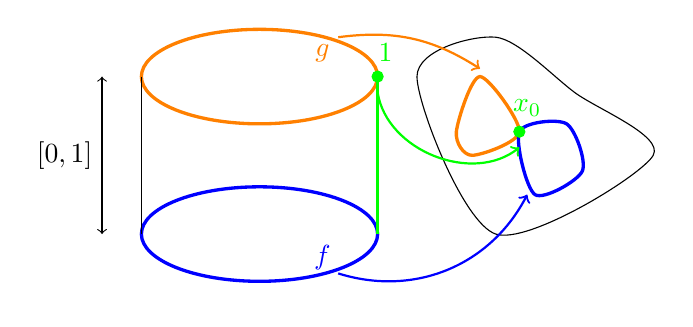
\begin{tikzpicture}
  \draw[orange, very thick] (-1, 1) ellipse (1.5 and 0.6);
  \draw[blue, very thick] (-1, -1) ellipse (1.5 and 0.6);

  \draw (-2.5, 1)--(-2.5, -1);
  \draw[green, very thick] (0.5, 1)--(0.5, -1);

  \filldraw[green] (0.5, 1) circle (2pt);
  \node at (0.6, 1.3) {$\color{green}1$};

  \draw[<->] (-3, 1)--(-3, -1) node [midway, left] {$[0,1]$};

  \draw[smooth cycle] plot coordinates {(1, 1) (2, 1.5) (3, 0.8) (4, 0) (2, -1)};
  \draw[smooth cycle, very thick, orange] plot coordinates {(2.3, 0.3) (1.8, 1) (1.5, 0.3) (1.7, 0)};
  \draw[smooth cycle, very thick, blue] plot coordinates {(2.3, 0.3) (2.9, 0.4) (3.1, -0.2) (2.5, -0.5)};
  \filldraw[green] (2.3, 0.3) circle (2pt);

  \node at (-0.2, 1.3) {$\color{orange}g$};
  \node at (-0.2, -1.3) {$\color{blue}f$};
  \node at (2.4, 0.6) {$\color{green}x_0$};

  \path[orange, thick, ->] (0, 1.5) edge[bend left=20] (1.8, 1.1);
  \path[blue, thick, ->] (0, -1.5) edge[bend right=40] (2.4, -0.5);
  \path[green, thick, ->] (0.5, 0.8) edge [bend right=60] (2.3, 0.1);
\end{tikzpicture}\end{center}

Grupa fundamentalna okręgu z wyróżnionym punktem jest izomorficzna z liczbami całkowitymi:
$$\Pi_1(S^1, 1)=\Z.$$

Mając dwie przestrzenie topologiczne $(X, x_0)$ i $(Y, y_0)$ oraz ciągłą funkcję między nimi $f$, mamy
\begin{center}\begin{tikzcd}[column sep=small, row sep=large]
  \Pi_1(X, x_0)\arrow[d, "\Pi_1(f)" left] & \left[\sigma\right] \arrow[l, phantom, sloped, "\ni"] \arrow[d, "\Pi_1(f)"] \\ 
  \Pi_1(Y, y_0) & \left[f\circ\sigma\right] \arrow[l, phantom, sloped, "\ni"]
\end{tikzcd}\end{center}

\end{example}

\begin{theorem}
  Każde ciągłe odwzorowanie $f:D^2\to D^2$ ma punkt stały.
\end{theorem}

\begin{proof}
  A raczej jego szkic.

  Załóżmy nie wprost, że istnieje funkcja ciągła $f:D^2\to D^2$, która nie posiada punktu stałego. 

  Możemy wówczas zdefiniować funkcję $F:D^2\to\partial D^2=S^1$, która punktowi $y\in D^2$ przypisuje punkt przecięcia wychodzącej z $f(y)$ przechodzącej przez $y$ z obwodem $D^2$:
  \begin{center}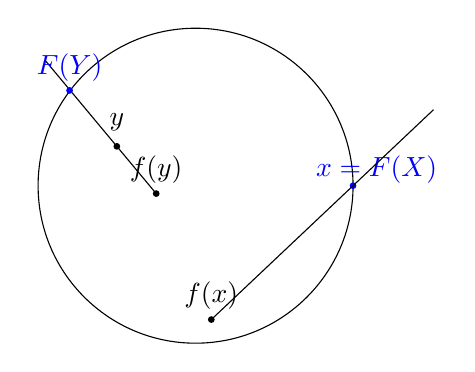
\begin{tikzpicture}
    \draw (0, 0) circle (2);

  \filldraw (-1, 0.5) circle (1pt);
  \node at (-1, 0.8) {$y$};

  \filldraw (-0.5, -0.1) circle (1pt);
  \node at (-0.5, 0.2) {$f(y)$};

  \draw[shorten <= -40pt] (-1, 0.5)--(-0.5, -0.1);
  \filldraw[blue] (-1.6, 1.21) circle (1pt);
  \node at (-1.6, 1.5) {$\color{blue}F(Y)$};


  \filldraw[blue] (2, 0) circle (1pt);
  \node at (2.3, 0.2) {$\color{blue}x=F(X)$};

  \filldraw (0.2, -1.7) circle (1pt);
  \node at (0.2, -1.4) {$f(x)$};

  \draw[shorten <= -40pt] (2, 0) -- (0.2, -1.7);
  \end{tikzpicture}\end{center}
  Obcięcie takiej funkcji do brzegu $\partial D^2$ daje oczywiście identyczność na $\partial D^2$ (punkt $x$ wyżej). Powstaje więc diagram
  \begin{center}\begin{tikzcd}
    S^1\arrow[rr, hookrightarrow]\arrow[dr, "id_{S^1}" below left] & & D^2 \arrow[dl, "F"] \\ 
                                  & S^1
  \end{tikzcd}\end{center}
  na który możemy nałożyć funktor $\Pi_1$:
  \begin{center}\begin{tikzcd}
    \Z=\Pi_1(S^1)\arrow[rr, hookrightarrow]\arrow[dr, "id_{\Z}=\Pi_1(id_{S^1})" below left] & & \Pi_1(D^2)=0 \arrow[dl, "\Pi_1(F)"] \\ 
                                  & \Pi_1(S^1)=\Z
  \end{tikzcd}\end{center}
  Czyli $\Z\to \Z$ faktoryzowałoby się przez $0$, a to jest niemożliwe.
\end{proof}

\begin{definition}[kategoria dualna]
  Dla kategorii $\mathbf{C}$ możemy zdefiniować nową kategorię, $\mathbf{C}^{op}$ w której każdy morfizm $\phi^{op}\in Hom_{\mathbf{C}^{op}}(Y, X)$ zostaje odwrócony:
  \begin{center}\begin{tikzcd}
    X\arrow[r, bend left=20, "\phi"] & Y\arrow[l, bend left=20, "\phi^{op}"]
  \end{tikzcd}\end{center}
  Wtedy $\ob\mathbf{C}^{op}$ to obiekty dualne do elementów znajdujących się w $\ob\mathbf{C}$. Tak zdefiniowaną kategorię $\mathbf{C}^{op}$ nazywamy \buff{kategorią dualną}.
\end{definition}

\begin{example}
\item Kategoria dualna do kategorii przestrzeni liniowych $\mathbf{Vect}_K^{op}$ jest kategorią, której obiekty to przestrzenie sprzężone, $V^*\in\ob\mathbf{Vect}^{op}_K$, zawierające funkcjonały liniowe $V\to K$. Każdy morfizm $\phi:V\to W$ w $\mathbf{Vect}_K$ indukuje wówczas odwzorowanie $\phi^*:W^*\to V^*$ takie, że dla $f\in W^*$ mamy $\phi^*(f)=f\circ\phi:V\to W\to K$.

  Kojarzenie funkcjonału $\phi^*\in V^*$ z elementem $v\in V$ jest czasem oznaczane przez $\langle \phi, v\rangle=\phi(v)$.
\end{example}

\begin{definition}[funktor kontrawariantny]
  Funktor (kowariantny) z kategorii $\mathbf{C}^{op}$ do kategorii $\mathbf{D}$ jest nazywamy \buff{funktorem kontrawariantnym} z $\mathbf{C}$ do $\mathbf{D}$.
\end{definition}

Oznacza to, że jeśli $X,Y\in\ob\mathbf{C}$ i $\phi:X\to Y\in Hom_{\mathbf{C}}(X, Y)$, to funktor kontrawariantny $F:\mathbf{C}^{op}\to\mathbf{D}$ przeprowadza $X$ na $F(X)\in\ob\mathbf{D}$, a $\phi\mapsto F(\phi)\in Hom_{\mathbf{D}}(F(Y),F(X))$.
\begin{center}\begin{tikzcd}[column sep=large]
  X \arrow[d, "\phi" left] \arrow[r, "F", yshift=-5mm, xshift=1mm, rightsquigarrow] & F(X) \\ 
  Y \arrow[d, "\psi" left] \arrow[r, "F", yshift=-5mm, xshift=1mm, rightsquigarrow] & F(Y) \arrow[u, "F(\phi)" right] \\ 
  Z & F(Z) \arrow[u, "F(\psi)" right] 
\end{tikzcd}\end{center}
Składanie morfizmów również zmienia kolejność, tzn.
$$F(\psi\phi)=F(\phi)F(\psi)$$









%Niech $R$ będzie dowolnym pierścieniem, natomiast $A, B, C$ będą $R$-modułami. Mając ciąg
%
%\begin{center}\begin{tikzcd}
%  A\arrow[r, "f"] & B\arrow[r, "g"] & C
%\end{tikzcd}\end{center}
%
%mówimy, że jest on \acc{dokładny}, jeśli $\ker(g)=\img(f)$. W szczególności implikuje to, że $g\circ f=gf:A\to C$ jest homomorfizmem zerowym.
%
%\begin{definition}[Kompleks łańcuchowy]
%  Rozważmy rodzinę $C=\{C_n\}_{n\in\Z}$ $R$-modułów wraz z mapami $d=d_n:C_n\to C_{n-1}$ takimi, że każde złożenie
%  $$[d_{n-1}\circ d_n=]d\circ d:C_n\to C_{n-2}$$
%  jest zerowe. Wówczas każdą mapę $d_n$ nazywamy \buff{różniczkami $C$}, a rodzina $C$ jest \buff{kompleksem łańcuchowym}.
%\end{definition}
%
%Jądra każdego $d_n$ nazywamy \acc{$n$-cyklami} $C$ i oznaczamy $Z_n=Z_n(C)$, natomiast obraz każdego $d_{n+1}$ jest nazywany \acc{$n$-granicą} $C$ i oznacza się jako $B_n=B_n(C)$. Ponieważ $d_n\circ d_{n+1}=0$, to
%$$0\subseteq B_n\subseteq Z_n\subseteq C_n.$$
%
%\begin{definition}[Homologia]
%  \buff{$n$-tym modułem homologii} kompleksu $C$ nazywamy iloraz $\color{green}H_n(C)=Z_n/B_n$.
%\end{definition}
%
%\begin{problem}
%  Ustalmy $C_n=\Z/8$ dla $n\geq0$ i $C_n=0$ dla $n<0$. Dla $n>0$ niech $d_n$ posyła $x\mod 8$ do $4x\mod 8$. Pokaż, że tak zdefiniowane $C$ jest kompleksem łańcuchowym $\Z/8$-modułów i policz moduły homologii.
%\end{problem}
%
%\begin{solution}
%  Zauważyć, że $d_{n-1}d_n=0$ jest nietrudno dla $n\leq1$ ($d_{n-1}d_n:C_n\to C_{n-2}=0$). Z kolei dla dowolnego $n>1$ i dowolnego $x\in C_n$ wiemy, że $d_n(x)=4x\mod 8$. Jeśli $x$ było oryginalnie liczbą parzystą, to od razu widać, że $d_n(x)=0$. Z kolei gdy $x$ jest nieparzyste, to wówczas 
%  $$d_{n-1}d_n(x)=d_{n-1}(4x\mod 8)=16x\mod 8=8\cdot(2x)\mod 8=0,$$
%  a więc $d_{n-1}d_n=0$.
%
%  Homologie dla $n<2$ są trywialne, natomiast dla $n\geq 2$ wszystkie są takie same (gdyż funkcje $d_n$ jak i moduły $C_n$ nie ulegają zmianie wraz z $n$). Wystarczy więc przyjrzeć się $Z_1/B_1$
%  
%  \begin{center}\begin{tikzcd}
%    C_0=\Z/8 & C_1=\Z/8\arrow[l, "d_1"] & C_2=\Z/8\arrow[l, "d_2"]
%  \end{tikzcd}\end{center}
%
%  $Z_1$ to liczby parzyste w $\Z/8$ (kernel $d_1$), natomiast $B_1$ to liczby podzielne przez $4$, ale nie przez $8$ w $C_1$. W takim razie, $Z_1/B_1=\{4\}$.
%\end{solution}
